
\documentclass[tikz, border=10pt]{standalone}
\usepackage{tikz}
\usepackage{xcolor}

\begin{document}
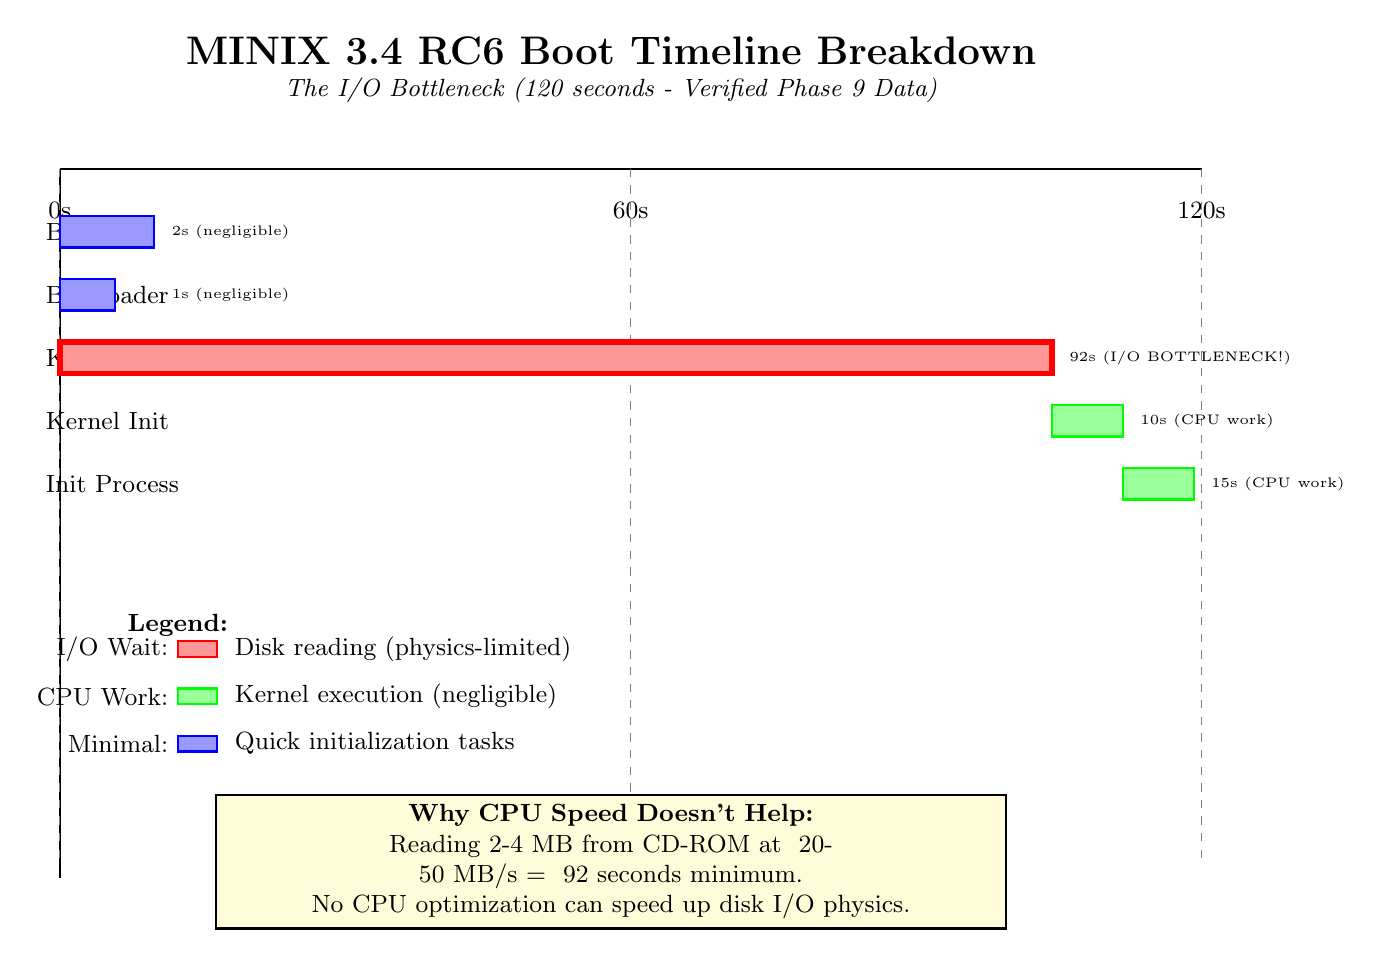
\begin{tikzpicture}[
    scale=1.0,
    font=\small,
]

% Title
\node[font=\Large\bfseries] at (7.5, 11.5) {MINIX 3.4 RC6 Boot Timeline Breakdown};
\node[font=\small\itshape] at (7.5, 11) {The I/O Bottleneck (120 seconds - Verified Phase 9 Data)};

% Axes
\draw[thick] (0.5, 10) -- (15, 10);
\draw[thick] (0.5, 10) -- (0.5, 1);

% Time axis labels
\node[below] at (0.5, 9.7) {0s};
\node[below] at (7.75, 9.7) {60s};
\node[below] at (15, 9.7) {120s};

% Grid lines
\foreach \x in {0.5, 7.75, 15} {
    \draw[thin, gray, dashed] (\x, 10) -- (\x, 1.2);
}

% Boot phase bars
\node[right] at (0.2, 9.2) {BIOS Init};
\draw[fill=blue!40, draw=blue, thick] (0.5, 9) rectangle (1.7, 9.4);
\node[font=\tiny, right] at (1.8, 9.2) {2s (negligible)};

\node[right] at (0.2, 8.4) {Bootloader};
\draw[fill=blue!40, draw=blue, thick] (0.5, 8.2) rectangle (1.2, 8.6);
\node[font=\tiny, right] at (1.8, 8.4) {1s (negligible)};

\node[right] at (0.2, 7.6) {Kernel Load};
\draw[fill=red!40, draw=red, thick, line width=2pt] (0.5, 7.4) rectangle (13.1, 7.8);
\node[font=\tiny, right] at (13.2, 7.6) {92s (I/O BOTTLENECK!)};

\node[right] at (0.2, 6.8) {Kernel Init};
\draw[fill=green!40, draw=green, thick] (13.1, 6.6) rectangle (14.0, 7.0);
\node[font=\tiny, right] at (14.1, 6.8) {10s (CPU work)};

\node[right] at (0.2, 6.0) {Init Process};
\draw[fill=green!40, draw=green, thick] (14.0, 5.8) rectangle (14.9, 6.2);
\node[font=\tiny, right] at (15.0, 6.0) {15s (CPU work)};

% Legend
\node[font=\small\bfseries] at (2, 4.2) {Legend:};
\draw[fill=red!40, draw=red, thick] (2, 3.8) rectangle (2.5, 4);
\node[left] at (2, 3.9) {I/O Wait:};
\node[right] at (2.6, 3.9) {Disk reading (physics-limited)};

\draw[fill=green!40, draw=green, thick] (2, 3.2) rectangle (2.5, 3.4);
\node[left] at (2, 3.3) {CPU Work:};
\node[right] at (2.6, 3.3) {Kernel execution (negligible)};

\draw[fill=blue!40, draw=blue, thick] (2, 2.6) rectangle (2.5, 2.8);
\node[left] at (2, 2.7) {Minimal:};
\node[right] at (2.6, 2.7) {Quick initialization tasks};

% Key insight
\node[draw, thick, rectangle, fill=yellow!15, minimum width=10cm, minimum height=1.2cm,
      text width=9.8cm, align=center] at (7.5, 1.2) {
    \textbf{Why CPU Speed Doesn't Help:}\\
    Reading 2-4 MB from CD-ROM at ~20-50 MB/s = ~92 seconds minimum.\\
    No CPU optimization can speed up disk I/O physics.
};

\end{tikzpicture}
\end{document}
